\chapter{Introduction}

\section{Long-Range Graph Learning as an Evaluation Problem}

Consider a target node whose binary label depends on a source node several edges away.
The source feature alone is not sufficient because the label also depends on the intermediate nodes along a source-to-target path.
A positive case contains the required feature pattern along that path, whereas a plausible negative case preserves the distant source and target but breaks the path condition at an intermediate node.
Distinguishing these cases for the intended reason requires a path-aware dependency rather than mere access to a distant node.

\begin{figure}[t]
\centering
\begin{minipage}[t]{0.49\textwidth}
\centering
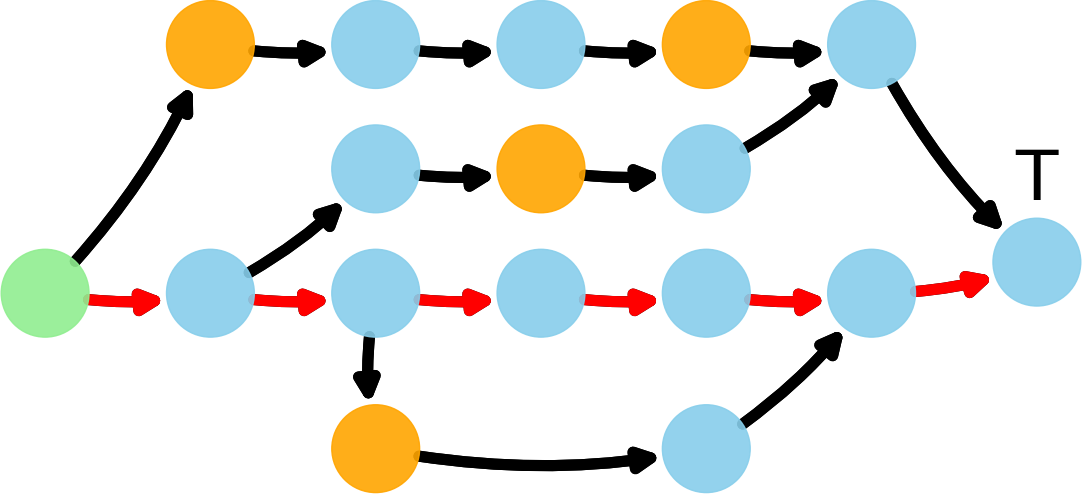
\includegraphics[width=\linewidth]{figures/glora-positive-d6.png}
\textbf{(a)} Positive example
\end{minipage}\hfill
\begin{minipage}[t]{0.49\textwidth}
\centering
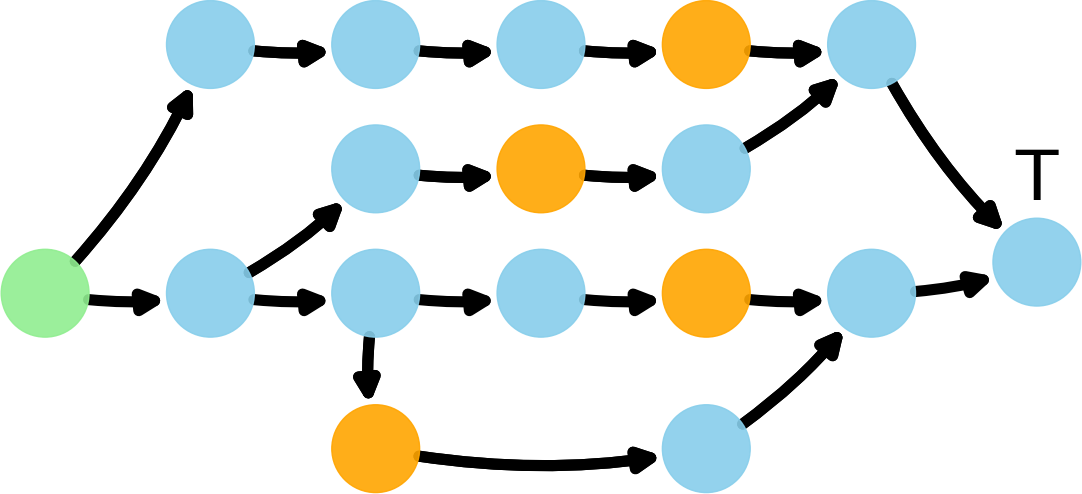
\includegraphics[width=\linewidth]{figures/glora-negative-d6.png}
\textbf{(b)} Negative example
\end{minipage}
\caption{A positive and a negative GLoRa example at generator parameter $d=6$.
Green nodes mark sources, blue nodes are normal nodes, orange nodes are holes, and $T$ marks the target node.
The red arrows identify the intended source-to-target chain; the negative example breaks this chain with a hole.
Adapted from Figure~1 of Paper~I \cite{zhou2025glora}.}
\label{fig:glora-running-example}
\end{figure}

This example also exposes an ambiguity in benchmark evidence.
A graph learning system may predict the labels from the source-to-target relation, or it may use a local marker or global statistic that happens to correlate with the labels.
Both functions can produce high accuracy on a dataset that permits the shortcut.
The score alone therefore does not show which function the system learned.

This distinction matters because graph learning is used when relations between objects carry information that isolated feature vectors omit.
Long-range relations arise in social influence and recommendation \cite{qiu2018deepinf,fan2019graph,liu2022social}, traffic and air-quality prediction \cite{li2021traffic,iskandaryan2023air}, internet safety and finance \cite{han2020fake,weber2018aml}, and biochemical prediction \cite{jha2022protein,bongini2022drugnn}.
These applications do not share one target function or one useful notion of distance.
They do share the need to establish whether a prediction used relevant information beyond the target node's immediate neighbourhood.

Message-passing graph neural networks provide the main technical setting for this problem \cite{scarselli2008graph}.
Their local updates make information from progressively more distant nodes available as layers are added.
Availability does not establish use: a source node may fall inside the receptive field while the learned prediction ignores the source-to-target path.
The modelling problem is to make the relevant information available and learnable, while the evaluation problem is to show that the learned function depends on it.

A benchmark for this purpose must specify the intended dependency and vary its length under controlled conditions.
It must also rule out shortcut functions, keep the target function expressible by the evaluated systems, and compare the two classes fairly.
Without these controls, success may overstate long-range ability and failure may reflect an inexpressible target rather than a learning limitation.

This thesis responds to that evaluation gap through GLoRa, the Graph Long-Range dependency benchmark introduced in the sole included paper \cite{zhou2025glora}.
GLoRa is a synthetic benchmark generator that treats dependency length as a controlled input to inductive binary node classification.
It addresses one family of path-aware dependencies and links a benchmark score to evidence about whether a system learned the specified dependency.
The thesis therefore uses GLoRa as a controlled evaluation method rather than only as a leaderboard.

\section{Scope and Research Questions}

The thesis has a deliberately narrow empirical scope.
It studies inductive binary node classification and one controlled family of path-aware dependencies.
Each example contains a graph, a target node, and a binary label, while the relevant evidence concerns a source-to-target relation of specified length.
The thesis does not claim that this setting represents every node-level, graph-level, or real-world long-range task.

The scope also separates quantities that can otherwise be conflated.
Graph size does not determine dependency length, and access at a large graph distance does not by itself demonstrate the intended dependency.
Later chapters distinguish the exact witness-path length from the implemented GLoRa generator parameter whenever their values differ.
Here, dependency length names the property under evaluation; it does not mean graph size or model depth.

The thesis does not infer a mechanism from an accuracy curve.
An accuracy trend is an observed symptom that requires separate diagnostic evidence before it supports a failure explanation.
Chapter 4 examines over-smoothing, over-squashing, and vanishing gradients as candidate explanations.

Within these boundaries, the thesis addresses three research questions.

\begin{description}
\item[RQ1:]
What evidence is required to conclude that a graph learning system has learned a path-aware dependency of a specified length?

\item[RQ2:]
How can a benchmark isolate a path-aware dependency of a specified length while ruling out shortcut functions, retaining target expressibility, and comparing systems fairly?

\item[RQ3:]
Under controlled evaluation, how does performance change with dependency length, and to what extent do the diagnostics support common failure explanations?
\end{description}

RQ1 defines the evidential claim, and RQ2 asks how an evaluation can support it.
RQ3 then asks what the resulting measurements establish within the tested setting.

\section{Contributions and Paper I}

This is an article-based thesis with one included paper.
Paper I is the thesis's sole empirical contribution and the paper around which the kappa is organised.

\begin{description}
\item[Paper I]
Dongzhuoran Zhou, Evgeny Kharlamov, and Egor V. Kostylev.
\emph{GLoRa: A Benchmark to Evaluate the Ability to Learn Long-Range Dependencies in Graphs}.
Published as a conference paper at ICLR 2025.
\end{description}

Dongzhuoran Zhou is the first author of Paper I.

The thesis makes three contributions through Paper I and the kappa.

\begin{enumerate}
\item \textbf{An evidence standard for path-aware long-range learning (RQ1).}
This contribution states what must be shown before a benchmark result supports a claim about a dependency of specified length.
It draws on GLoRa's path-aware definition and the locality, expressivity, and access-versus-use analysis in Chapters 2 and 3 \cite{zhou2025glora}.

\item \textbf{A controlled benchmark for the stated dependency family (RQ2).}
GLoRa is a generator for evaluating inductive binary node classification across controlled dependency lengths.
Its construction and formal guarantees define the path-aware dependency, rule out shortcut functions under the stated conditions, establish target expressibility, and specify the fairness conditions \cite{barcelo2020logical,zhou2025glora}.

\item \textbf{A controlled comparison and diagnostic assessment across dependency lengths (RQ3).}
This contribution compares graph learning systems under controlled conditions and assesses candidate failure explanations.
It combines experiments indexed by dependency length with separate diagnostics for over-smoothing, over-squashing, and vanishing gradients in Paper I \cite{zhou2025glora}.
\end{enumerate}

These contributions stop at the tested systems, protocol, and path-aware dependency family.
They do not provide a universal account of long-range graph learning or identify a general cause of failure.

\section{Research Questions, Chapters, and Evidence}

Table~\ref{tab:introduction-rq-evidence} maps each research question to the chapters that develop it and to the corresponding form of evidence in GLoRa.

\begin{center}
\centering
\begin{tabular}{L{0.12\textwidth}L{0.40\textwidth}L{0.34\textwidth}}
\hline
\textbf{RQ} & \textbf{Kappa chapters} & \textbf{Evidence from GLoRa} \\
\hline
RQ1 & Chapters 2 and 3 & GLoRa definition \\
RQ2 & Chapters 5 and 6 & Construction, Properties~(P1)--(P3), length control, and protocol controls \\
RQ3 & Chapters 4 and 6 & Length-indexed performance and diagnostics \\
\hline
\end{tabular}
\captionsetup{hypcap=false}
\captionof{table}{Research questions, kappa chapters, and evidence from GLoRa.}
\captionsetup{hypcap=true}
\label{tab:introduction-rq-evidence}
\end{center}

For RQ1, Chapter 2 establishes when local message passing can access distant information, and Chapter 3 states what would demonstrate use of a path-aware dependency.
GLoRa's path-aware definition fixes the dependency to which this evidence standard applies.

For RQ2, Chapter 5 derives the benchmark requirements from threats to interpretation, and Chapter 6 shows how the GLoRa construction addresses those requirements.
The construction and its formal guarantees cover controlled dependency length, the stated shortcut exclusions, target expressibility, and class-distribution fairness; separate evaluation controls provide system-protocol fairness.

For RQ3, Chapter 4 states what evidence candidate explanations require, and Chapter 6 presents the length-indexed experiment and the corresponding diagnostics.
The performance trend is therefore only a symptom; the diagnostic measurements provide the evidence for assessing an explanation.

\section{Thesis Structure}

Chapter 2 establishes the graph-learning foundations needed to interpret a claim about long-range use, including local message passing, receptive fields, and expressivity.
Chapter 3 then distinguishes reachable information from information used by a prediction and develops the path-aware evaluation target and evidence standard for RQ1.

Chapter 4 identifies the diagnostic trace required for each candidate failure explanation.
Chapter 5 reviews whether existing evaluations control shortcut functions, target expressibility, fair comparison, and dependency length.

Chapter 6 presents GLoRa's construction, experiments, and diagnostics for RQ2 and RQ3.
Chapter 7 answers the three research questions, then discusses limitations and future work within the same evidence boundaries.
